
\chapter{显著性区域检测基础}
在本章中,将分类介绍几种国际上主流的几类显著区域检测方法:基于局部对比度(MZ\cite{ma2003contrast}),基于全局对比度(HC,RC\cite{cheng2011global}),基于频域分析(SR\cite{hou2007saliency}),基于学习(CRF\cite{maisaliency})。在本章的最后,还将介绍近年来的一些最新的工作和研究趋势。

\section{基于局部对比度的方法}
\begin{figure}[h]
\centering
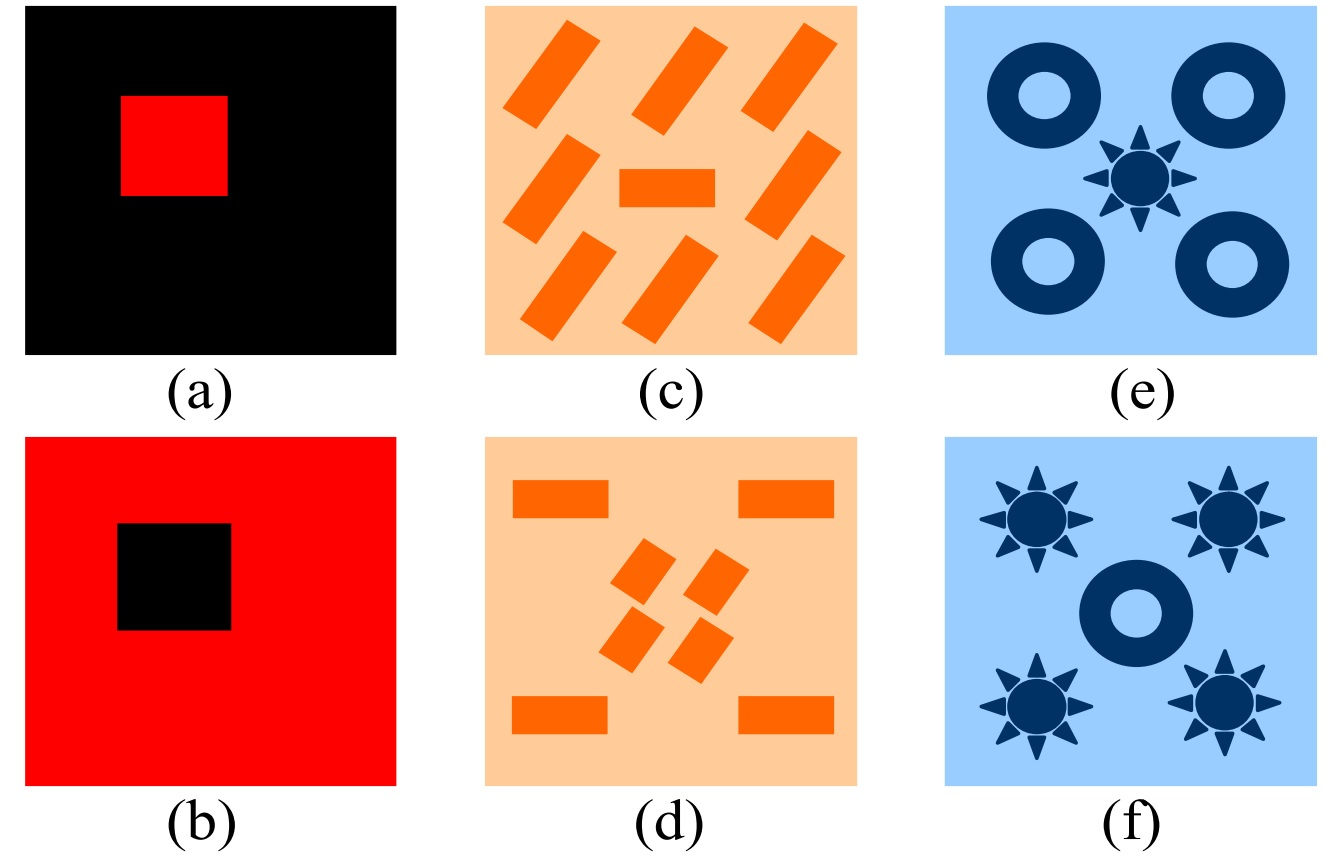
\includegraphics[width=\textwidth]{local_contrast.jpg}
\caption{对比度在视觉感知中的作用}\label{fig:local_contrast}
\end{figure}
传统的图像处理技术通常只考虑了颜色、纹理和形状这三个基本特征,然而,对比度在视觉感知中的重要作用却常常被人们所忽略。以下这个例子可以说明对比度的重要性\citep{ma2003contrast},如图\ref{fig:local_contrast}所示的三组合成图像,在图\ref{fig:local_contrast}(a)中,有一个红色的方形盒子被黑色的背景所围绕。很显然,红色盒子所在区域更容易吸引人们的注意力,对这个现象的一个解释是,因为红色是一种更容易引起人们视觉注意力的鲜艳色彩。然而,图\ref{fig:local_contrast}(b)却无法支持这个假设,显然在这幅图像中,黑色的区域却成为了吸引人们注意力的区域。这个现象表明,尽管颜色能够影响人们的视觉感知,但是却并非影响视觉注意力最重要的因素。图\ref{fig:local_contrast}(c)(d) 展示了两幅有一定纹理方向的图像,类似(a)(b)两图,说明了纹理并非视觉感知中最重要的因素。图\ref{fig:local_contrast}(e)(f)则说明了形状在视觉感知中的作用。然而,以上三组图像都有一个共同的特征,那就是,显著区域通常被背景区域围绕并呈现高对比度(无论是颜色、纹理还是形状上的高对比度),这在一定程度上说明了高对比度的物体通常能吸引人眼的注意力。基于局部对比度的方法利用了图像区域相对于(一个小的)局部邻域的稀缺度来检测显著性区域。在此定义下,检测子的形式通常表现为“中心-周围差异”,不同方法的变化在于:1)尺度问题(即“中心-周围差异”中,“周围”的大小);2)差异的度量问题(在哪种特征空间下比较、周围像素点的权值等)。本节以MZ\cite{ma2003contrast}方法为例,介绍基于局部对比度的方法。在MZ中,局部对比度被定义为:
\begin{equation}
C_{i,j} = \sum_{q \in \Theta}d(p_{i,j},q) \label{eq:local}
\end{equation}
其中$c_{i,j}$代表在$(i,j)$位置的像素点的对比度,$p_(i,j)$代表该像素点的某种特征向量(例如颜色向量),$q$代表周围像素点的特征向量,$d(x,y)$表示$p_{i,j}$与$q$的差异,通常使用欧式距离度量,$\Theta$即代表周围像素点的集合,通过控制$\Theta$的大小,即可控制“感知域”的大小。最后,将所有图像的对比度的值normalize到0,1之间,即得到像素的显著值。可以看出,这个定义下,一个像素点的显著值实际上就是它与周围像素点的差异和。

实际上,对这个公式做一些变形,就可以衍生出其他的方法:1)调整$\Theta$的范围,就可以调整检测子的尺度。近期的一些工作,已经不满足于通常的矩形或圆形邻域,开始寻找一些特性更好的邻域(比如邻域边界与图像边缘一致的邻域)。2)改换特征空间,比如在梯度空间下,或者其他自定义的特征空间。3)加入权值,公式\ref{eq:local}认为周围像素点对中心像素点的贡献是一样的,权值都为1,但是实际上,与中心像素点距离近的像素可能对其对比度的贡献更高,所以可以对距离中心近的像素点赋更大的权值。

以上就是基于局部对比度的显著区域检测方法的核心。然而,这种方法有一个很严重的问题,它倾向于给物体边缘赋予较大的显著值,因为物体边缘的“中心-周围差异度”通常较大。在尺度选的较小时,检测子实际上已经近似退化为一个边缘检测子。

\section{基于全局对比度的方法}
在上一节提到,基于局部对比度的方法,倾向于给物体边缘赋予较大的显著值,而无法均匀的高亮整个显著区域。为了解决这个问题,研究者想到采用全局对比度计算显著图。相比基于局部对比度的方法,基于全局对比度的方法就不存在只高亮边缘的问题,因为在全局环境下(即将像素点的邻域扩展到全图),具有相同特征的像素(如颜色)必然赋予相同的显著值。实际上,早在2006年,Zhai\cite{zhai2006visual}等人就已经提出了全局对比度这个概念,只是当时他们考虑到计算复杂度的问题,仅仅采用了像素的亮度值来计算像素点之间的差异。显然,用一个像素点的亮度值来度量像素点之间的相似性是非常粗糙的,比如纯红和纯蓝的亮度值是一样的,但是这两个颜色显然有着很大的差别。因此,在Cheng的工作中\cite{cheng2011global},使用了颜色的三个通道进行计算。在HC方法中,一个像素点$I_k$的显著值定义为:
\begin{equation}
S(I_k)=\sum_{\forall I_i \in I}D(I_k,I_i)
\end{equation}
其中$I$代表整个图像像素点的集合,$I_i$代表第$i$个像素点在Lab颜色空间的颜色向量,$D(*,*)$为欧式距离算子。很明显,在这个公式中,颜色相同的像素肯定会得到相同的显著值,为了进一步减少计算开销,上式可以进一步简化为:
\begin{equation}
S(I_k)=S(c_l)=\sum_{j=1}^n f_j D(c_l,c_j)
\end{equation}
其中$c_l$代表像素$I_k$的颜色向量,$c_j$代表第$j$个颜色的颜色向量,$f_j$代表第$j$种颜色在整个图像中出现的频率。经分析可知,计算上式的时间复杂度为$O(N)+O(n^2)$,$N$为像素的个数,$n$为整个图像中不同颜色的数量。如果不经过任何优化,原颜色空间的颜色个数为$n=256^3$,显然这样的时间复杂度是不可忍受的。因此,Cheng首先将每个颜色通道量化为12个值,这样颜色的数量下降为$n=12^3=1728$。
\begin{figure}
\centering
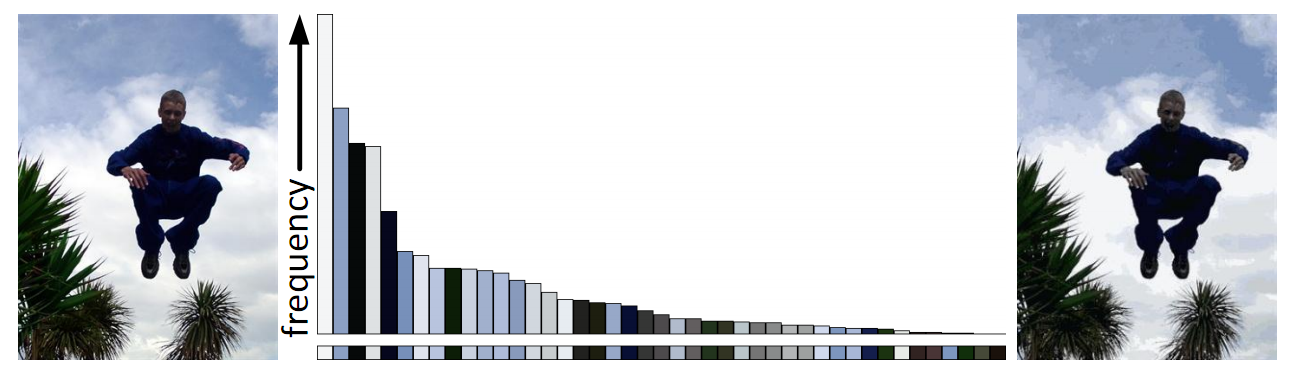
\includegraphics[width=\textwidth]{global_contrast.png}
\caption{使用少量高频颜色量化图像}\label{fig:global_contrast}
\end{figure}
进一步的,如图\ref{fig:global_contrast}所示,忽略占像素数量较少的颜色,使用出现频率高的颜色替代,使得剩余的颜色占到像素数量的$95\%$,颜色的数量可以进一步下降到$85$左右(忽略的颜色使用剩余颜色中最相近的代替),同时基本不影响图像的主观视觉质量\cite{cheng2011global},这样就大大降低了时间复杂度。然而,如此量化后,会给图像带来很明显的量化痕迹,比如原本非常相近的两个颜色,可能会被量化到不同的值。因此,为了优化效果,Cheng最后还使用了一个颜色空间的平滑,即对相近颜色的显著值进行了加权平均,.具体做法如下:
\begin{equation}
S'(c) = \frac{1}{(m-1)T}\sum_{i=1}^{m}(T-D(c,c_i))S(c_i)
\end{equation}
其中$T=\sum_{i=1}^m D(c,c_i)$是颜色$c$与最相近的m种颜色的距离和。文章中还介绍了RC方法,即Region Based Contrast,该方法首先使用一般的分割方法将图像分割为许多区域,然后使用该区域的平均颜色作为区域的颜色值,最后使用相似的方法,以区域为基本计算单元,计算区域的全局对比度。

\section{基于频域分析的方法}
基于频域分析的方法主要将图像转化到频域处理,并结合信息压缩理论,将图像中“新颖”的频率部分分离出来,最后再转回空间域。这里以SR\cite{hou2007saliency}为例子进行分析。在信息压缩理论中,一幅图像的信息量可以被分解为两部分:
\begin{equation}
H(Image)=H(Innovation)+H(Prior Knowledge)
\end{equation}
对于$H(Prior knowledge)$是我们已知的一些先验知识,所以可以不用编码,只需对$H(Innovation)$这部分进行编码传输即可。解码时,由于先验知识已知,我们通过解码$H(Innovation)$这部分,就可以恢复原图像,从而达到信息压缩的目的。而显著性区域即对应$H(Innovation)$这部分内容,这也是基于频域处理方法的理论基础。

\begin{figure}[h]
\centering
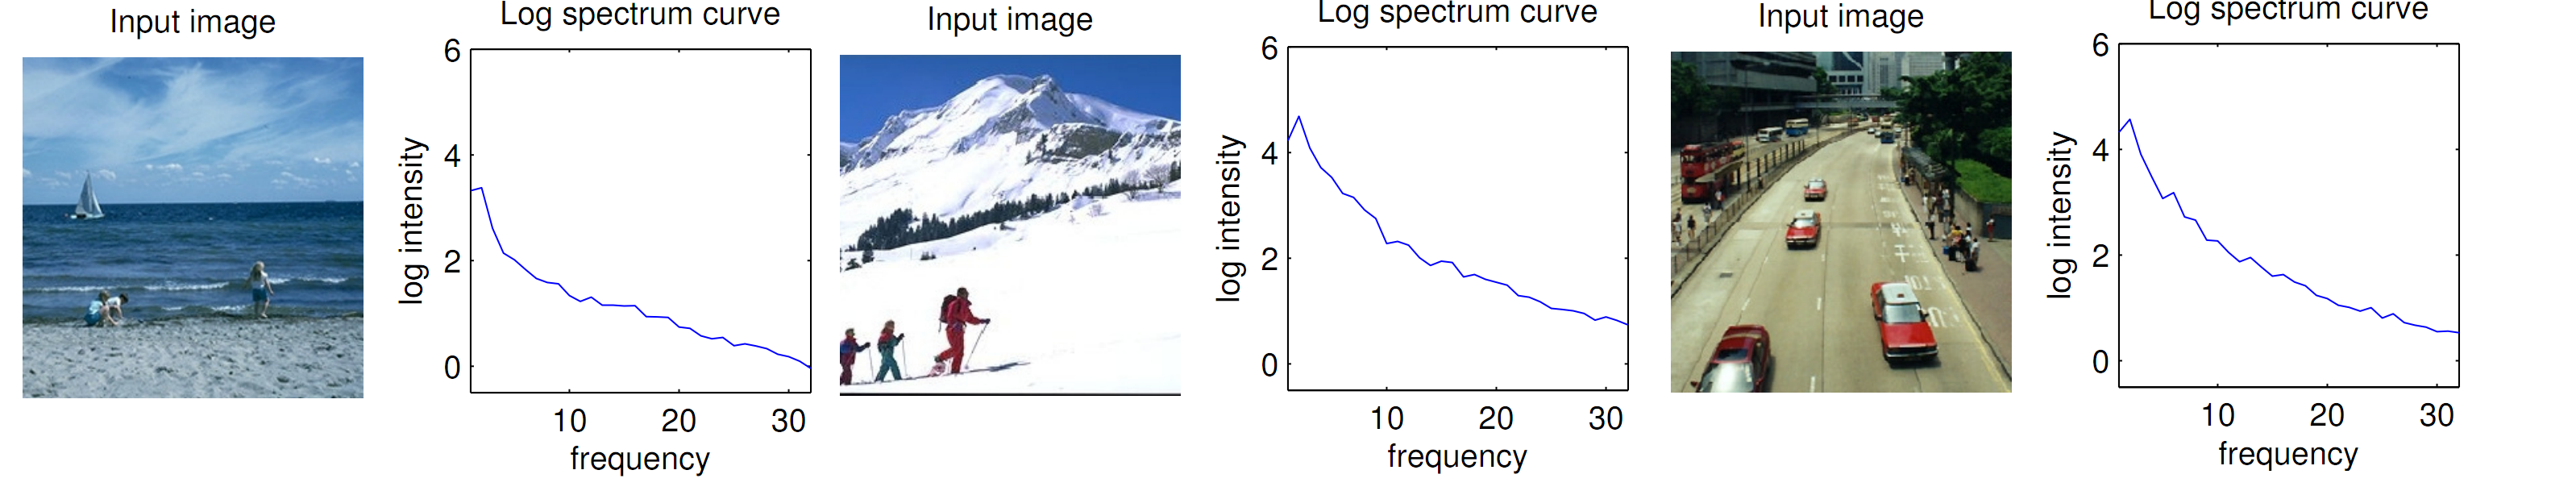
\includegraphics[width=\textwidth]{log_spectrum.png}
\caption{不同图像的log spectrum呈现为相似的曲线}\label{fig:log_spectrum}
\end{figure}

\begin{figure}[t]
\centering
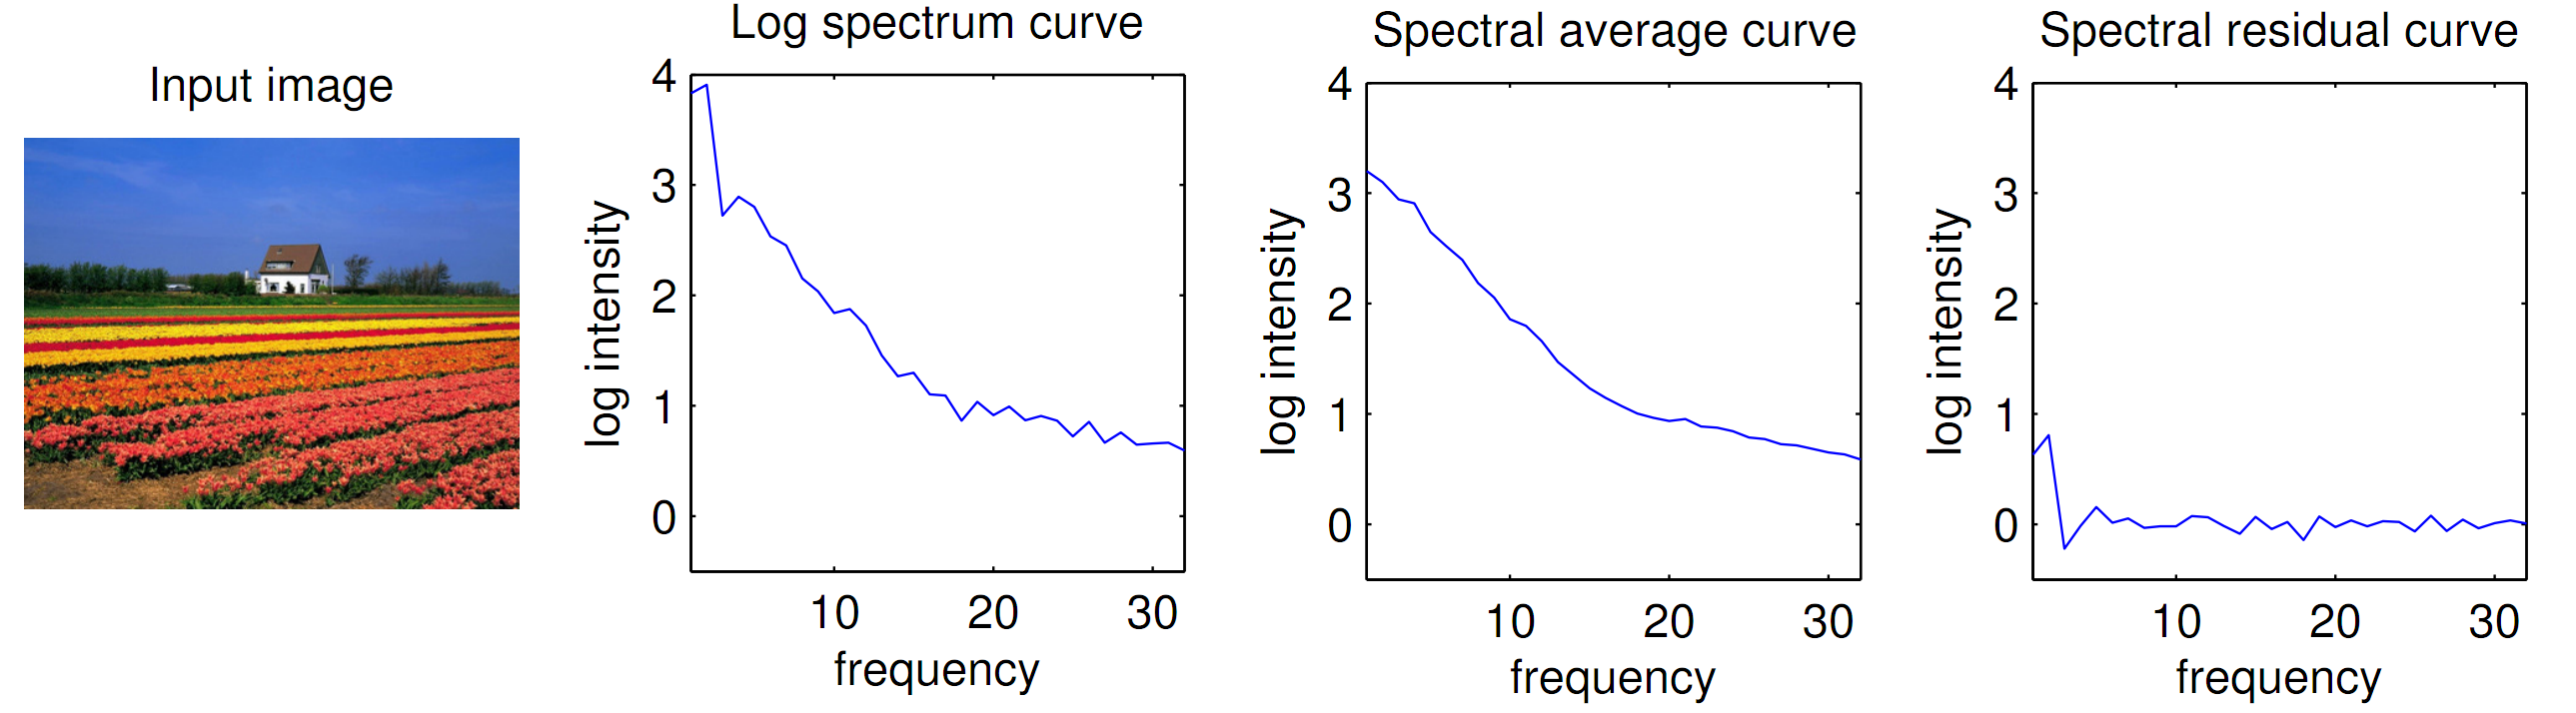
\includegraphics[width=\textwidth]{frequency_residual.png}
\caption{通过求得log spectrum的残差得到显著区域}\label{fig:frequency_residual}
\end{figure}

文章指出,图像的log spectrum具有相似的变化曲线,如图\ref{fig:log_spectrum}所示,这也就是对应的先验知识,因此通过求得一大批图像log spectrum曲线的均值,我们就可以得到图像在频率域的“先验知识”。如图\ref{fig:frequency_residual},将图像的log spectrum减去先验,得到的残差,即为显著区域对应的频域的表达,再通过逆变化,变换到时域,即可得到显著图。

然而有文章\cite{hou2012image}指出,这些基于频域分析的方法实际上等同于基于局部对比度的方法加上一个高斯模糊,因此与基于局部对比度的方法具有相同的缺陷,即容易高亮物体的边缘。

\section{基于学习的方法}
这里介绍Mai等人\cite{maisaliency}提出的使用条件随机场(CRF)的模型。作者基于这样的观察:既然现在有这么多的显著区域检测方法,而且不同的方法针对不同的场景都会有一定的效果,那么如果能够将这些方法结合起来,肯定能够互相补充,得到更好的结果。如图\ref{fig:crf_learn}所示,(c)(d)(e)(f)四种方法均能取得一定的效果,但是都有各自的缺陷,比如(f)只高亮了显著区域的边缘,而(e)方法对显著和非显著区域的区分不明显,而通过CRF结合多种方法相互补充,可以看到CRF-GIST方法可以取得很好的效果。实际上,这个思想在Itti的学生Borji的一篇文章中\cite{borji2012salient}就已经涉及到了,只是在Borji的文章中,结合多种特征的方式比较简单,即采用简单的加权平均,或者对应像素相乘等等。Mai等人指出\cite{maisaliency},简单的相加相乘并没有考虑到相邻像素之间的关联性,即如果能加入空间位置信息(相邻且相似的像素的显著性应该比较接近),应该能取得更好的效果。

\begin{figure}[h]
\centering
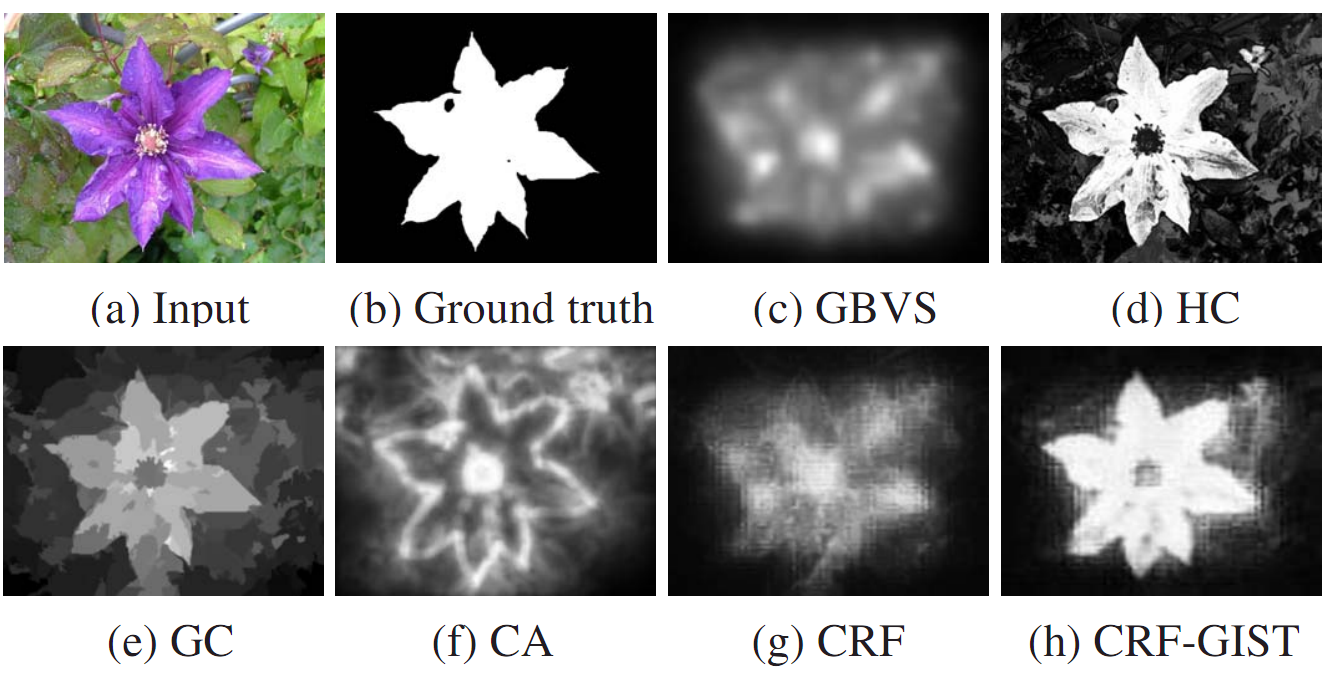
\includegraphics[width=\textwidth]{crf_learn.png}
\caption{结合多个显著图}\label{fig:crf_learn}
\end{figure}

在Mai的模型中,给定一幅图像$I$,我们使用一个二值掩图$Y=\{y_p|p\in I\}$来标出显著物体。在CRF模型中,以每个像素点为顶点,8领域像素点之间相连,形成一个晶格状的图。那么,在这个图下,$Y$在给定图像$I$下的条件概率可以写为,
\begin{equation}
P(Y|I) = \frac{1}{Z}exp(\sum_{p\in I}F_d(y_p, I) + \sum_{p\in I}\sum_{q\in N_p}F_s(y_p,y_q,I) )
\end{equation}
其中$p$代表$I$中的一个像素点,$y_p$是其显著与否的标记。$F_d(y_p, I)$是node feature function,$F_s(y_p,y_q,I)$是edge feature function,描述了相邻像素点之间的联系。

Node feature function仅仅与输入的已有显著图$S_i$有关,即
\begin{equation}
F_d(y_p, I) = \sum_{i=1}^{m} \lambda_iS_i(p) + \lambda_{m+1}y_p
\end{equation}
其中$\lambda_i$是条件随机场的一组待学习的参数。Edge feature function描述了相邻像素之间的关系:
\begin{equation}
F_s(y_p,y_q,I) = F_e(y_p,y_q,I) + F_c(y_p,y_q,I)
\end{equation}
其中$F_e(y_p,y_q,I)$考虑到了这样一个事实,如果两个像素点在同一幅显著图中的显著值差别很大,那么他们最后倾向于拥有不同的显著性标记。
\begin{equation}
  F_e(y_p,y_q,I) = \sum_{i=1}^{m}\alpha_i(\textbf{1}(y_p=1,y_q=0)-\textbf{1}(y_p=0,y_q=1))(S_i(p)-S_i(q))
\end{equation}
其中$\alpha_i$为CRF的待学习参数,$\textbf{1}(.)$为指示函数(括号内真为1,假为0)。$F_s$的第二项可以看做一个惩罚项,当像素点的颜色相似却被标上不同的标记时要进行惩罚:
\begin{equation}
F_c(y_p,y_q,I)=\textbf{1}(y_p \not= y_q) exp(-\beta \parallel I(p)-I(q) \parallel )
\end{equation}
其中$\parallel I(p)-I(q) \parallel$代表像素$p$和$q$的颜色差(Lab颜色空间),$\beta$被设置为$(2<\parallel I(p)-I(q) \parallel>^2)^{-1}$,$<.>$代表计算期望。

最后,通过训练这个模型,得到所有参数的最优值。当计算新的显著图时,我们取每个顶点(像素点)被标记为1的概率作为该像素点的显著值。

可以看出,基于学习的方法原理较为复杂,同时学习与训练比较耗时。另外,\citep{liu2011learning}指出,基于学习的方法比较依赖训练数据集,因此在不同的数据集合上,表现差异较大。

\section{最新工作与研究趋势}
除了以上一些经典的方法,近年来在该领域也出现了许多新颖且实用的工作\cite{borji2012salient}\cite{yan2013hierarchical}\cite{shi2013pisa}\cite{wei2012geodesic},大家对显著性区域检测的研究方向有了如下一些共识和趋势:
\begin{itemize}
\item 多尺度,多特征的融合。在小尺度下,一些很小的,对比度又很大的区域很容易影响到整个图像的显著性检测,而在大尺度下,则可以屏蔽这些区域,但是检测的粒度又会变得粗糙。因此,通过结合多个尺度,可以大大提高检测的精度和鲁棒度。对于多特征,前面已经说过,单一的特征都有其适用范围,不可能对于所有情况都有效,因此结合多个特征(颜色,纹理等等)可以使之互补。
\item 趋向于基于区域的特征。基于点的特征比较敏感,很容易受到噪声点的影响。最近的一些工作,基本都是基于区域的特征。尤其值得注意的是,大多使用了SLIC\cite{achanta2010slic}这个超像素分割算法,将空间上近似的像素点分割为一个小的区域进行计算。
\item 加入一些更高层的特征。底层的特征在简单场景下有良好的效果,但是在复杂场景下往往会失效,加入高层特征(如人脸识别子,汽车识别子等等)有助于改善结果。
\item 将时间复杂度作为一项重要的考察指标。显著性区域检测的价值在于将其与其他应用相结合,单独的使用显著性区域检测算法没有任何意义。作为一项预处理技术,其时间复杂度决定了其实用性。
\end{itemize}

\section{本章小结}
本章介绍了显著性区域检测的四类经典算法:基于局部对比度、基于全局对比度、基于频域分析和基于学习的方法。基于局部对比度的方法符合人类对生物视觉的认知,然而却容易高亮区域边缘;基于全局对比度的方法则改良了上述缺点,能较好的高亮整个显著区域;基于频域分析的方法拥有良好的理论基础,但是其处理效果同基于局部对比度的方法一样,容易强调边缘的显著度;最后基于学习的方法能有效的结合各类特征,得到良好的效果,但是其训练时间过长,且与数据相关。在本章的最后,还介绍了国际上关于该课题最新的一些思路和研究趋势,这为我们未来的工作指明了方向。
